A Budapest School alternatív kerettanterv a többcélú, egységes	Budapest School Általános Iskola és Gimnázium számára készült, amely 12 évfolyammal működő nevelési-oktatási intézményként ellátja az általános iskola és a gimnázium feladatait.

A kerettanterv a köznevelésről szóló 2011.~évi CXC. törvény 9§ (8)--(9) bekezdésének felhatalmazása alapján a Budapest School iskola köznevelési tevékenységét a motiváció \citep{pink2011drive}\footnote{Az irodalomjegyzéket lásd a \pageref{sec:bibliographyk}. oldalon}, a fejlődési szemlélet \citep{growthmindset} és az elmélyült gyakorlás \citep{ericsson2016peak} pszichológiai kutatási eredményei, az  OECD, azaz a Gazdasági Együttműködési és Fejlesztési Szervezet \emph{Az iskolázás a jövőben}  (\emph{Schooling for Tomorrow}) programjának eredményei \citep{2006schooling} és a modern tanulásszervezési paradigmák, mint az önvezérelt \citep{mitra2012beyond} és a személyre szabott \citep{khan2012one} tanulás alapján határozza meg.

A kerettanterv a köznevelési törvény által megengedett területeken él a speciális szabályozás lehetőségével: meghatározza az iskola tanulásszervezési folyamatát, az értékelő/visszajelző rendszerét és szervezeti-működési sajátosságait. Ezek részeként bemutatja a pedagógus-munkakört, a pedagógusok végzettségével és szakképzettségével kapcsolatos követelményeket, a Budapest School	egyedi helyiség- és felszereléshasználati szabályait, az egy központi iskolával és több telephellyel működtetett mikroiskola-hálózati modellt és a Budapest School minőségfejlesztési alapelveit.

A kerettanterv egyszerre akar a gyerekek számára egy önvezérelt és személyreszabott tanulási környezetet biztosítani, ami képes agilisen reagálni a gyerekek és a környezet igényeire és egy stabil, biztonságos, kiszámítható rendszert is adni, ami biztosítja az iskola és más iskolák közötti átjárhatóságot, a továbbtanulást. Ezt a két szándékot ötvözi \aref{fig:bps_model}.~ábrán látható Budapest School modell.

\begin{figure}
    \centering
    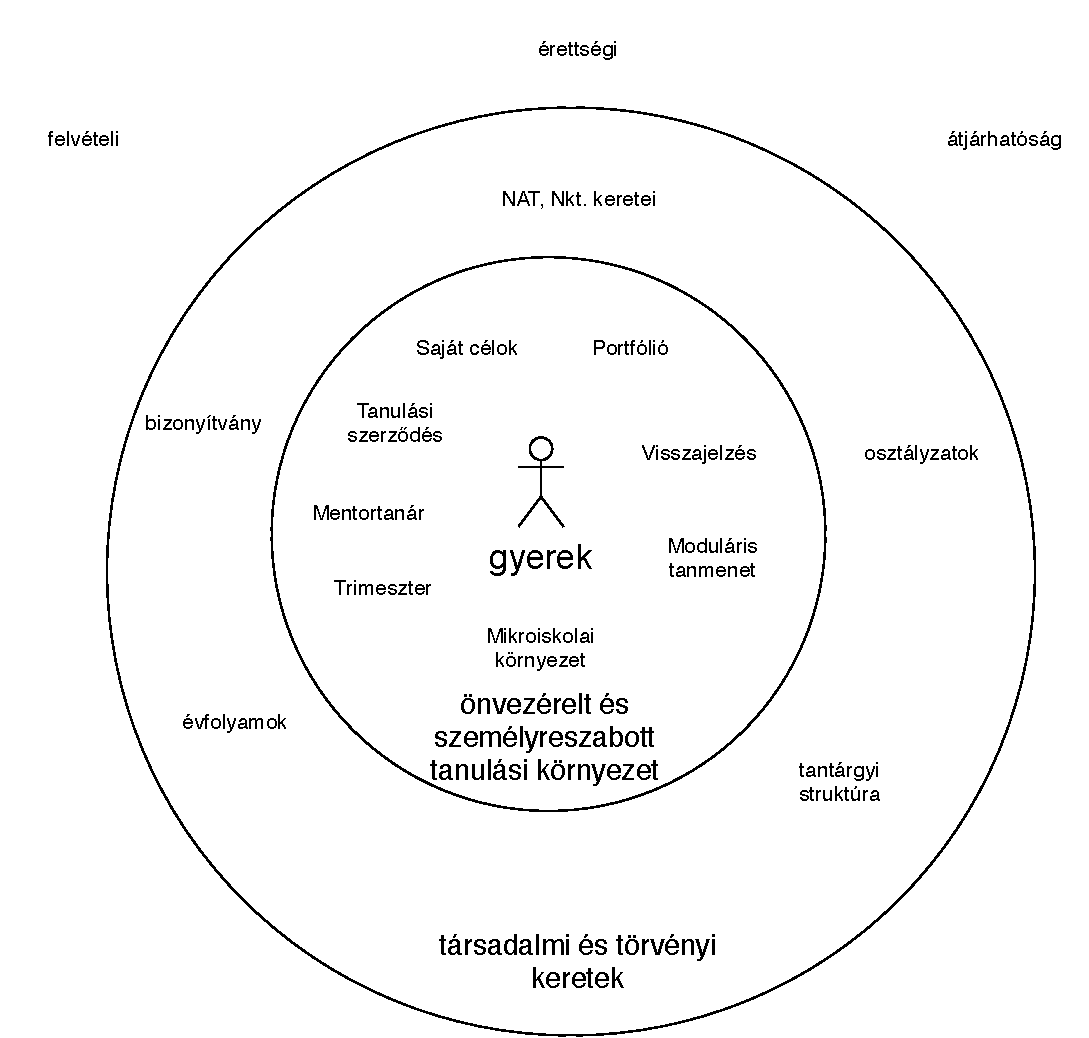
\includegraphics[width=0.8\textwidth]{chapters/kerettanterv/model.pdf}
    \caption{A Budapest School modellben a gyerek körüli buborékban szinte minden a gyerekről és az ő kisközösségéről szól. A külső kör képviseli a társadalmi, törvényi illeszkedést, átjárhatóságot.}
    \label{fig:bps_model}
\end{figure}

\paragraph{Kerettantervünk elsődleges célja} A kerettanterv bemutatja, hol, milyen módon, kitől és mit tanulhat egy Budapest Schoolba járó gyerek.
A gyerekek igényeire gyorsan reagáló mikroiskola egy buborék a gyerek körül. Ebben a körben a kerettanterv a tanulás folyamatát szabályozza, a \emph{mit tanulunk?} kérdés mellett a \emph{hogyan szervezzük meg a tanulást?} kérdésre ad választ. A tanulás során a gyerekek a kerettantervben részletezett módon az érdeklődésüknek megfelelően specifikus tanulási egységeket, vagyis modulokat végeznek el, melyek eredményeit a saját portfóliójukban gyűjtik össze. Így a gyerekek tanulási útja a portfólió fejlődésével nyomon követhető, és a portfólió tartalma alapján megállapítható a gyerek aktuális tudása, képessége. Az iskola fő funkciója emellett mindvégig az aktív tanulás, saját fejlődésük kereteinek megtalálása, a folyamatosan újragondolt saját célok állítása, és e célok irányába történő haladás marad.
 
A Budapest School kerettanterve a gyerekek, tanárok és a szülők közös döntésére bízza, hogy a gyerekek mit és hogyan tanulnak a kerettantervben meghatározott kereteken belül. A kerettanterv a specifikus célkitűzés-tervezés, a tanulás, és az arra történő reflektálás módját írja le, vagyis a tanulás folyamatát rögzíti, míg annak pontos tartalmában szabadságot enged.

\paragraph{A kerettanterv másodlagos célja}  Ennek a szabadságnak a \emph{kereteit} adja meg, hogy biztosítva legyen a mikroiskolán kívüli boldogulása is a gyerekeknek. A kerettanterv
 tantárgyi specifikációja a miniszter által kiadott kerettantervekre \citep{ofi:kerettanterv} épül, azokat strukturálja újra úgy, hogy megtartja annak tantárgyi struktúráját. A kerettanterv a tantárgyak tartalmát tanulási eredmények halmazaként adja meg. A tanulási eredmények féléves bontása, és a tantárgyi specifikációk lehetővé teszik a személyreszabott portfóliók osztályzatokra váltását egy átlátható folyamaton keresztül.

A tantárgyak lefedik a Nemzeti alaptanterv kiadásáról, bevezetéséről és alkalmazásáról szóló 110/2012. (VI. 4.) Korm. rendeletben leírt (a továbbiakban: NAT) műveltségi területeket, fejlesztési célokat és kulcskompetenciákat, 100\%-ban megfelelnek a miniszter által kiadott kerettantervek tantárgyi struktúrájának és az óraszámok is kevesebb mint 30\%-ban térnek csak el. A félévenkénti osztályzatok biztosítják az átjárhatóságot és a továbbtanuláshoz szükséges feltételeket. A kettős rendszer, a személyre szabott belső buborék és a kiszámíthatóságot adó külső kör biztosítja, hogy a 12.~évfolyam végén a gyerekeknek lehetőségük van arra, hogy érettségi vizsgát tegyenek.

\paragraph{Pedagógia módszerek}
A kerettantervünk semleges a pedagógiai módszerekkel kapcsolatban, a tanár feladatának tekinti, hogy mindig az optimálisnak tűnő tanulási, tanítási, gyakorlási módszert válassza. Ezért ez a kerettanterv nem beszél arról, hogy a modulokat (foglalkozásokat, tanórákat) milyen pedagógiai módszer alapján szervezi a tanár.

A kerettantervünk az iskolába járókat gyerekeknek hívja, nem tanulóknak és nem diákoknak. Ennek fő oka, hogy a rendszerünkben a tanárok és a szülők is tanulók, sőt az egész iskola egy tanuló szervezet, így a kerettanterv nem akarja  kizárólag az iskola egyik szereplőjére alkalmazni ezt a szót. Másodsorban a kerettanterv hangsúlyozza, hogy a \emph{család} fontos szerepet kap a Budapest School rendszerében: az iskolában a szülők, a gyerekek és a tanárok együttműködésben dolgoznak a fejlődésért. Azok a gyerekek, akik tanulmányaik vége felé felnőtté érnek a Budapest Schoolban, tanulók is maradnak, és talán egy kicsit gyerekek is, ezért a szóhasználaton miattuk sem változtatunk. Az ő esetükben a gyerek az iskolába járó tanulót jelenti.

\section{Az iskola célja}
\label{sec:iskola_celja}

A Budapest School abban támogatja a gyerekeket, hogy azok az
attitűdök, képességek és szokások alakuljanak ki bennük, amelyek segítségével
boldog, egészséges és a társadalom számára hasznos felnőttekké válhatnak. A
cél, hogy a gyerekek a mai világ szükségleteihez és lehetőségeihez a saját
erősségeik felhasználásával kapcsolódhassanak.	Hogy tanulási útjukat
sajátjukként éljék meg, és felelősséget érezzenek az alakításáért, az újabb és
újabb kihívások megtalálásáért.

Olyan tanulási környezetet kell kialakítani ehhez, ahol a szülők, tanárok és
gyerekek tesznek magukért és egymásért, ahol gyerekeink képesek nehéz
helyzetekben is életük, kapcsolataik és környezetük aktív alakítói lenni,
cselekedeteikkel, tetteikkel elérni a kitűzött céljaikat.

Mindenki kíváncsinak születik, és meg tudja tanulni azt, amit
igazán szeretne. Nincs is másra szükség, csak izgalmas kihívásokra, kérdésekre,
biztonságra, támogatásra és lehetőségekre.

Ennek szellemében az iskolánk elsődleges feladata, hogy a gyerekek közösségét
segítsék abban, hogy sokat és hatékonyan tanuljanak és alkossanak.
\emph{Tanulják azt, amit szeretnének, és azt, amire szükségük van.}

